%&..\preamble

\def\npart {IA}
\def\nterm {Michaelmas}
\def\nyear {2021}
\def\nlecturer {A.\ Chailinor}
\def\ncourse {Differential Equations}
\def\nauthor{Author}

\def\encodingdefault{TU}\normalfont
\ifnum 0\ifxetex 1\fi\ifluatex 1\fi=0 % if pdftex
  \usepackage[T1]{fontenc}
  \usepackage[utf8]{inputenc}
  \usepackage{textcomp} % provide euro and other symbols
\else % if luatex or xetex
  % \usepackage{unicode-math}
  % \defaultfontfeatures{Scale=MatchLowercase}
  % \defaultfontfeatures[\rmfamily]{Ligatures=TeX,Scale=1}
  % \DeclareMathAlphabet{\mathcal}{OMS}{cmsy}{m}{n}
  % \let\mathbb\relax % remove the definition by unicode-math
  % \DeclareMathAlphabet{\mathbb}{U}{msb}{m}{n}
\fi

\usetikzlibrary{external}
\tikzset{external/system call={xelatex -fmt=../preamble.fmt \tikzexternalcheckshellescape -halt-on-error -interaction=batchmode -jobname "\image" "\texsource"}} % path is relative to file that includes preamble
\tikzexternalize

\providetoggle{DontSetTitleAuthorDate}

\nottoggle{DontSetTitleAuthorDate}{
  \hypersetup{
    pdftitle={Part \npart\ - \ncourse},
    pdfsubject={Cambridge Maths Notes: Part \npart\ - \ncourse},
    pdfkeywords={Cambridge Mathematics Maths Math \npart\ \nterm\ \nyear\ \ncourse}
  }

  \author{Based on lectures by \nlecturer}
  \date{\nterm\ \nyear}
  \title{Part \npart\ --- \ncourse}
}{}

\tikzsetexternalprefix{figtemp/}

\begin{document}
\maketitle

\section{Syllabus}


{\small
  \noindent\textbf{Basic calculus}\\
  Informal treatment of differentiation as a limit, the chain rule, Leibnitz's rule, Taylor series, informal treatment of $O$ and $o$ notation and l'H\^opital's rule; integration as an area, fundamental theorem of calculus, integration by substitution and parts.\hspace*{\fill}[3]

  \vspace{5pt}
  \noindent Informal treatment of partial derivatives, geometrical interpretation, statement (only) of symmetry of mixed partial derivatives, chain rule, implicit differentiation. Informal treatment of differentials, including exact differentials. Differentiation of an integral with respect to a parameter.\hspace*{\fill}[2]

  \vspace{10pt}
  \noindent\textbf{First-order linear differential equations}\\
  Equations with constant coefficients: exponential growth, comparison with discrete equations, series solution; modelling examples including radioactive decay.

  \vspace{5pt}
  \noindent Equations with non-constant coefficients: solution by integrating factor.\hspace*{\fill}[2]

  \vspace{10pt}
  \noindent\textbf{Nonlinear first-order equations}\\
  Separable equations. Exact equations. Sketching solution trajectories. Equilibrium solutions, stability by perturbation; examples, including logistic equation and chemical kinetics. Discrete equations: equilibrium solutions, stability; examples including the logistic map.\hspace*{\fill}[4]

  \vspace{10pt}
  \noindent\textbf{Higher-order linear differential equations}\\
  Complementary function and particular integral, linear independence, Wronskian (for second-order equations), Abel's theorem. Equations with constant coefficients and examples including radioactive sequences, comparison in simple cases with difference equations, reduction of order, resonance, transients, damping. Homogeneous equations. Response to step and impulse function inputs; introduction to the notions of the Heaviside step-function and the Dirac delta-function. Series solutions including statement only of the need for the logarithmic solution.\hspace*{\fill}[8]

  \vspace{10pt}
  \noindent\textbf{Multivariate functions: applications}\\
  Directional derivatives and the gradient vector. Statement of Taylor series for functions on $\mathbb{R}^n$. Local extrema of real functions, classification using the Hessian matrix. Coupled first order systems: equivalence to single higher order equations; solution by matrix methods. Non-degenerate phase portraits local to equilibrium points; stability.

  \vspace{5pt}
  \noindent Simple examples of first- and second-order partial differential equations, solution of the wave equation in the form $f(x + ct) + g(x - ct)$.\hspace*{\fill}[5]}

\tableofcontents

\setcounter{section}{-1}

\hypertarget{introduction-video}{%
\section{Introduction Video}\label{introduction-video}}

24 lecture course. 
Full notes will be provided on moodle, small typefont indicates an aside, either because the material is non examinable or will be covered in greater detail in a later course.

Four example sheets.

\hypertarget{schedule}{%
\subsection{Schedule}\label{schedule}}

\begin{enumerate}
\def\labelenumi{\arabic{enumi}.}
\tightlist
\item
  Basic Calculus (5 lectures)
\item
  First-order linear differential equations (2)
\item
  Nonlinear first-order differential equations (4)
\item
  Higher-order linear differential equations (8)
\item
  Multivariate functions: applications (5)
\end{enumerate}

\hypertarget{introduction}{%
\subsection{Introduction}\label{introduction}}

They describe the rate of change of the \textcolor{red}{dependent variable} wrt the \textcolor{red}{independent variable}.

\begin{example}[Newton's 2nd law] ~\vspace*{-1.5\baselineskip}
\begin{align*}
  m \frac{d^2 x}{d t^2} = F
\end{align*}
If \(F\) depends only on \(t\), then we can simply integrate twice. However, if \(F\) is a function of \(x\) (such as a charged particle in a electric field which varied over space).
\end{example}

\textbf{Applied course} - emphasises \textcolor{red}{methods} and \textcolor{red}{results} rather than \textcolor{red}{proof} or \textcolor{red}{existence}.

\hypertarget{limits}{%
\subsection{Limits}\label{limits}}

\begin{itemize}
\item
  Informally, if \(\lim_{x \to x_0} f(x) = A\), then \(f(x)\) can be made arbitrarily close to \(A\) by making \(x\) sufficiently close to \(x_0\)

  \begin{itemize}
  \tightlist
  \item
    Note, does not require \(f(x_0)\) to equal \(A\) (or even to exist) -- a limit is a statement about the behaviour of a function in the vicinity of \(x_0\), but not at that point.
  \end{itemize}
\item
  More formally, for a function \(f(x)\) defined on some open interval containing \(x_0\) (but not necessarily at \(x_0\)), \(\lim_{x \to x_0} f(x) = A\) means that

  \begin{itemize}
  \tightlist
  \item
    for any \(\epsilon > 0\), there exists \(\delta >0\) such that \(|f(x) - A| < \epsilon\) for all \(0 < |x - x_0| < \delta\).
  \item
    Right hand limit, for example, defined similarly but with \(0 < |x - x_0| < \delta\) replaced with \(0 < x - x_0 < \delta\). A similar procedure can be done for left hand limits
  \end{itemize}

  \begin{figure}[h!]
    \centering 
    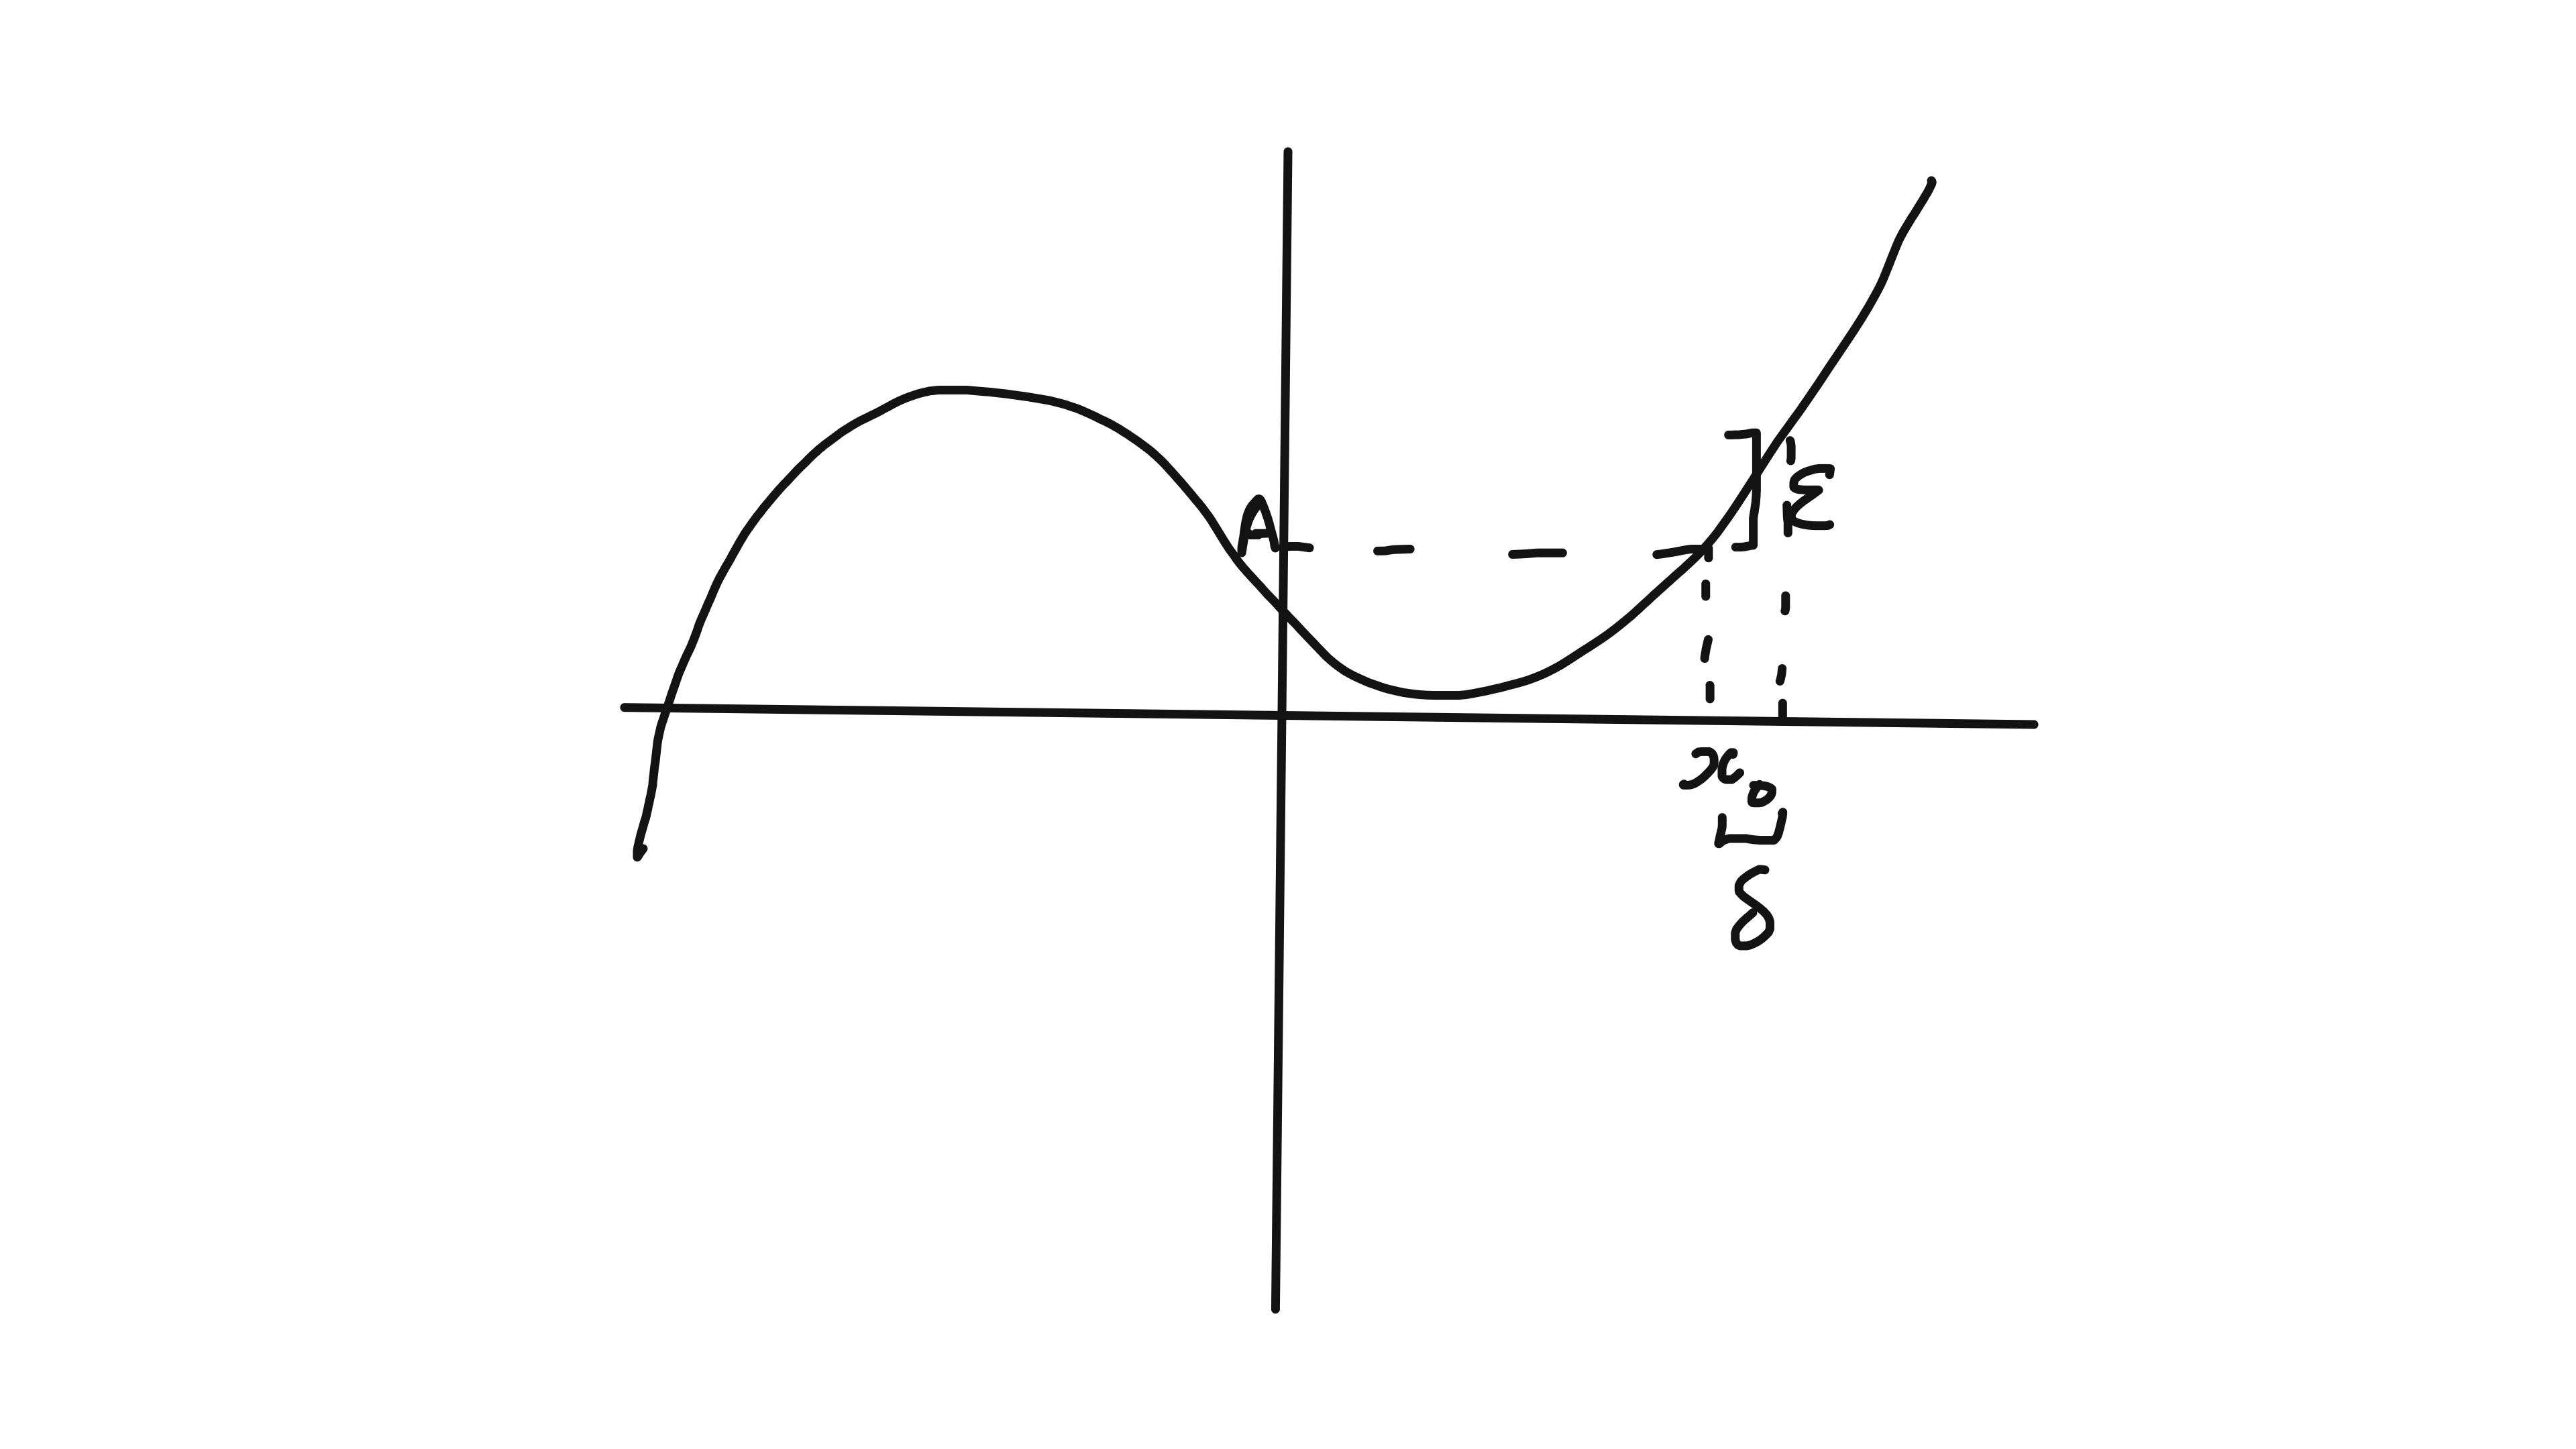
\includegraphics{figures/1}
    \caption{Right hand limit}
  \end{figure} \label{fig:1}
  
\item
  We can also define limits at infinity, e.g.~\(\lim_{x \to x_0} f(x) = A\) means that

  \begin{itemize}
  \tightlist
  \item
    for any \(\epsilon > 0\), there exists \(X >0\) such that \(|f(x) - A| < \epsilon\) for all \(x > X\).
  \end{itemize}
\end{itemize}

\hypertarget{properties}{%
\subsubsection{Properties}\label{properties}}

\begin{itemize}
\tightlist
\item
  If \(f(x)\) has a limit at a point, it is unique
\item
  If \(\lim_{x \to x_0} f(x) = A\) and \(\lim_{x \to x_0} g(x) = B\), then:

  \begin{itemize}
  \tightlist
  \item
    \(\lim_{x \to x_0} [f(x) + g(x)] = A + B\)\\
  \item
    \(\lim_{x \to x_0} [f(x)g(x)] = AB\)\\
  \item
    \(\lim_{x \to x_0} [f(x) / g(x)] = A / B\). If \(B = 0\), the limit of the quotient does not exist if \(A \neq 0\), but \textcolor{red}{may} exist in the \textcolor{red}{indeterminate} case \(A = B = 0\)
  \end{itemize}
\end{itemize}

These properties will be proved carefully in the Analysis 1 course next term, but will be used as without proof in this course.

\hypertarget{proof-of-uniqueness-of-limits}{%
\subsubsection{Proof of uniqueness of limits}\label{proof-of-uniqueness-of-limits}}

Suppose that \(\lim_{x \to x_0} f(x) = A\) \textcolor{red}{and} \(\lim_{x \to x_0} f(x) = B\).
In terms of our epsilon-delta definition, this means that for any \(\epsilon > 0\) there exists \(\delta_A > 0\) and \(\delta_B > 0\) such that
\begin{align*}
  &\text{for }0 < |x -x_0| < \delta_A,\ |f(x) - A| < \epsilon / 2 \text{, where } \epsilon / 2 \text{ is an arbitrary positive quantity.} \\
  \color{red}{and} \ &\text{for } 0 < |x -x_0| < \delta_A,\ |f(x) - B| < \epsilon / 2
\end{align*}
Now let \(\delta = min(\delta_A, \delta_B)\) and consider \(0 < |x -x_0| < \delta\) - follows that
\begin{align*}
  |A - B| &= |[A - f(x)] - [B - f(x)]| \\
  &\leq |A - f(x)| + |B - f(x)| \\
  &\leq \epsilon
\end{align*}
Since this holds \textcolor{red}{for all} \(\epsilon > 0\), we must have \(A = B\).

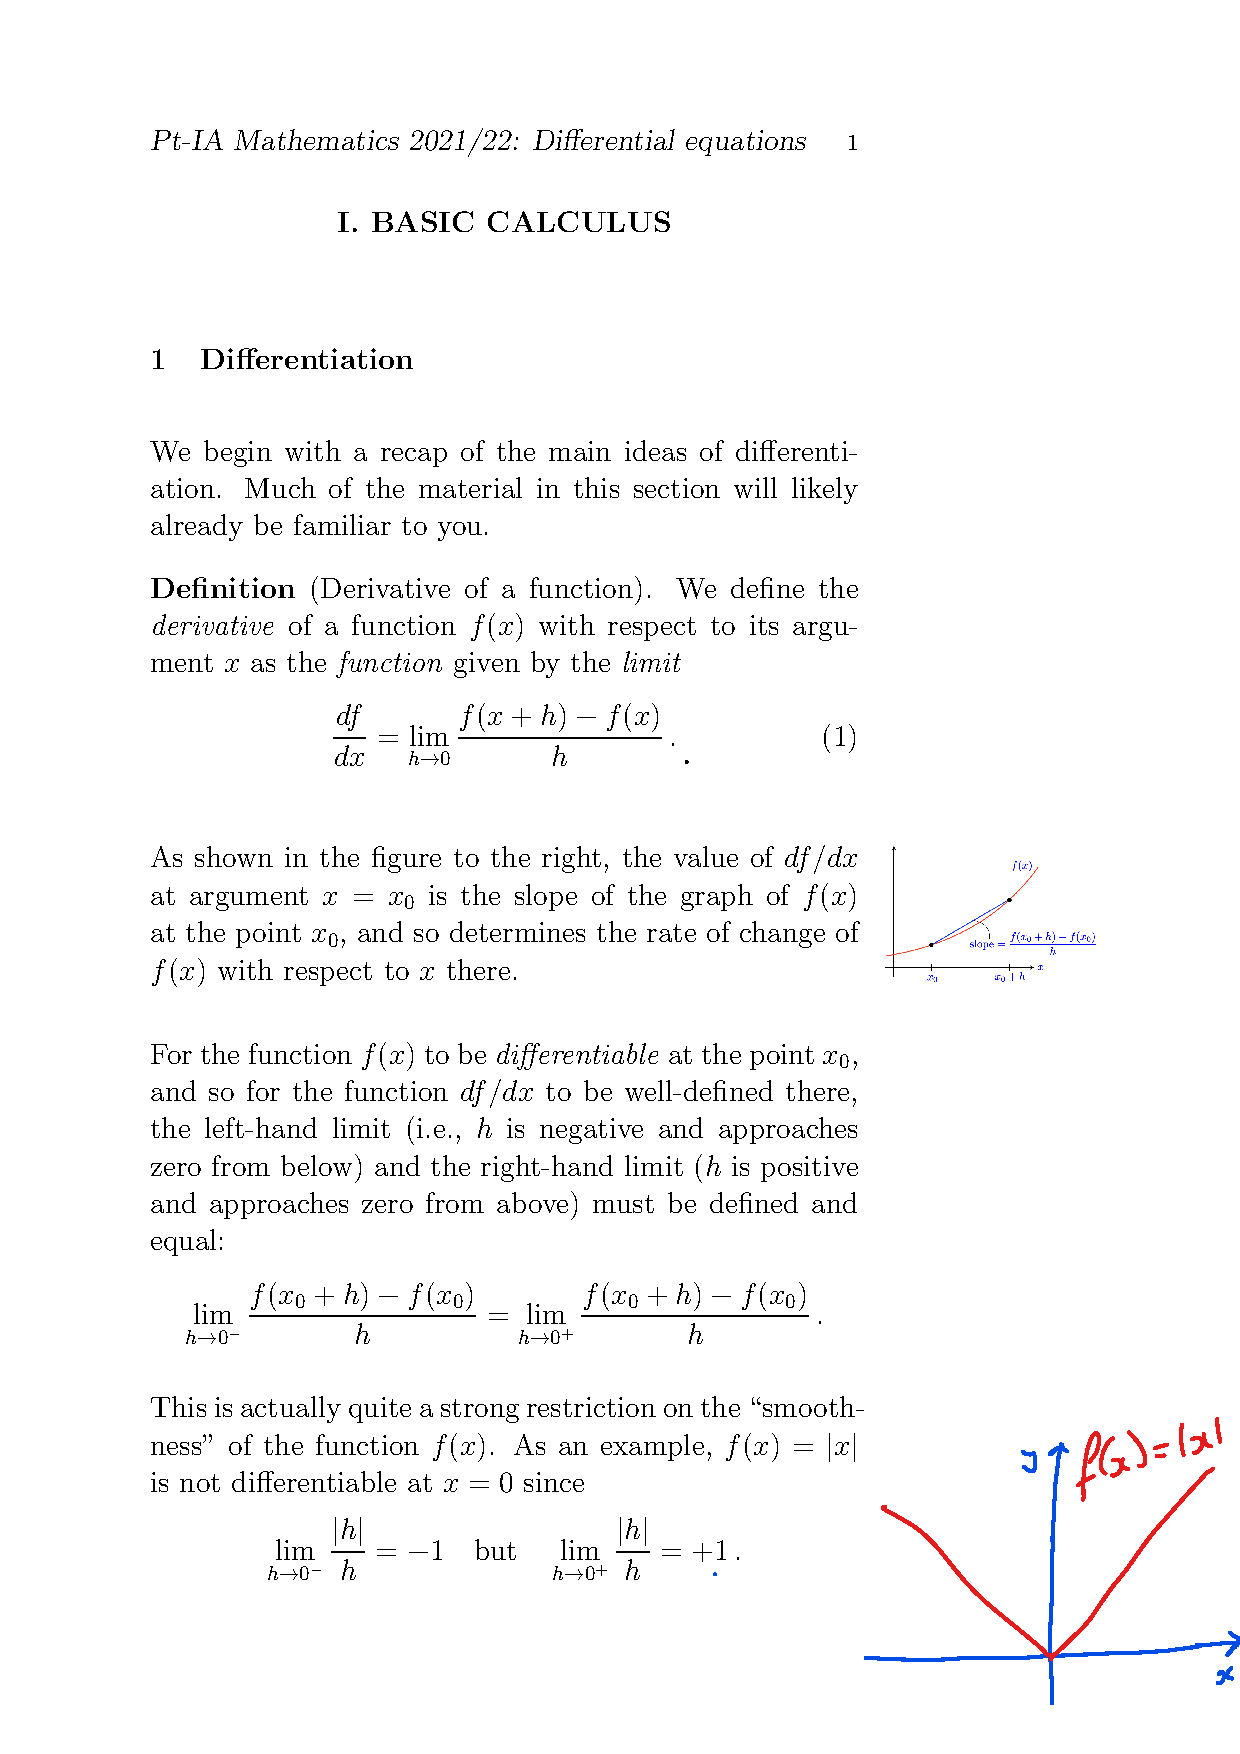
\includepdf[pages=-, addtotoc={ 1,section,1, Basic Calculus,1}]{Basic Calculus - Topic 1.pdf}

\subsection{Extra}

If \(f(x) = o(g(x))\) as \(x \to x_0\), then \(af(x) = o(g(x))\) as \(x \to x_0\) for finite \(a\).

\emph{Aside}: (Non examinable)

\begin{proof}[Sketch proof of Taylor's Theorem]
Start from FTC
\begin{align*}
    \int_{0}^{x} f'(t) \,dt &= f(x) - f(0) \\
    \implies f(x) &= f(0) + \int_{0}^{x} f'(t) \,dt \\
    &= f(0) + \int_{0}^{x} \frac{d (t - x)}{d t} * f'(t) \,dt \\
    &= f(0) + [ (t - x) f'(t)]^{t = x}_{t = 0} - \int_{0}^{t} (t - x) f''(t) \,dt \\
    &= f(0) + xf'(0) - \frac{1}{2} \int_{0}^{t} \frac{d (t-x)^2}{d t} f''(t) \,dt \\
    &= f(0) + xf'(0) - \frac{1}{2} [(t-x)^2 f''(t)]^{t = x}_{t = 0} - \int_{0}^{t} + \frac{1}{2} \int_{0}^{t} (t - x)^2 f'''(t) \,dt \\
    &= f(0) + xf'(0) + \frac{1}{2} x^2 f''(0) + \frac{1}{2} \int_{0}^{t} (t - x)^2 f'''(t) \,dt \\
    &\;\;\vdots \\
    &= f(0) + xf'(0) + \frac{x^2}{2!} f''(0) + \ldots + \frac{x^n}{n!} f^{(n)}(0) + \frac{1}{n!} \int_{0}^{x} (t - x)^n f^{(n + 1)}(t) \,dt \\
    &\text{By MVT the remainder = somehow} \\
    &= \frac{x^{(n+1)}}{(n + 1)!} f^{(n + 1)}(x_n) \text{ where } x_n \in [0, x]
\end{align*}
\end{proof}


(q12, sheet 1)

i. 
\begin{align*}
    p(V, S): \\
    dp &= \left. \frac{\partial p}{\partial V} \right|_S dV + \left. \frac{\partial p}{\partial S} \right|_V dS \\
    \text{Actually } S &= S(V, T) \\
    \text{so, } dS &= \left. \frac{\partial S}{\partial V} \right|_{T} dV + \left. \frac{\partial S}{\partial T} \right|_{V} dT \\
    \implies dp &= \left( \left. \frac{\partial p}{\partial V} \right|_{S} + \left. \frac{\partial p}{\partial S} \right|_{V} \left. \frac{\partial S}{\partial V} \right|_{T} \right) dV + \left. \frac{\partial p}{\partial S} \right|_{V} \left. \frac{\partial S}{\partial T} \right|_{V} dT
\end{align*} 

ii. \begin{align*}
    \text{We want } \left. \frac{\partial U}{\partial V} \right|_{T} \text{ and } \left. \frac{\partial U}{\partial T} \right|_{V} : U(V, T) \\
    \text{We are given } dU &= TdS - pdV \\
    &= \underbrace{T \left. \frac{\partial S}{\partial T} \right|_{V}}_{\equiv \left. \frac{\partial U}{\partial T} \right|_{V}} dT + \underbrace{ \left( T \left. \frac{\partial S}{\partial V} \right|_{T} - p \right)}_{\equiv \left. \frac{\partial U}{\partial V} \right|_{T}} dV
\end{align*} 

\textbf{3.4.3 Differentiation of an integral with respect to its parameters}

\begin{example}
Suppose we want to evaluate
\begin{align*}
    \int_{0}^{\infty} x^n e^{-x} \,dx \text{ where n is an integer} \\
    \text{Let } I(\lambda) = \int_{0}^{\infty} e^{-\lambda x} \,dx = \frac{1}{\lambda} \\
    \frac{d^n}{d \lambda^n} I = \int_{0}^{\infty} (-x)^n e^{-\lambda x} \,dx = (-1)^n \frac{n!}{\lambda^{n + 1}} \\
    \text{set } \lambda = 1 \text{ and we get } \int_{0}^{\infty} x^n e^{-x} \,dx = n!
\end{align*}
\end{example}

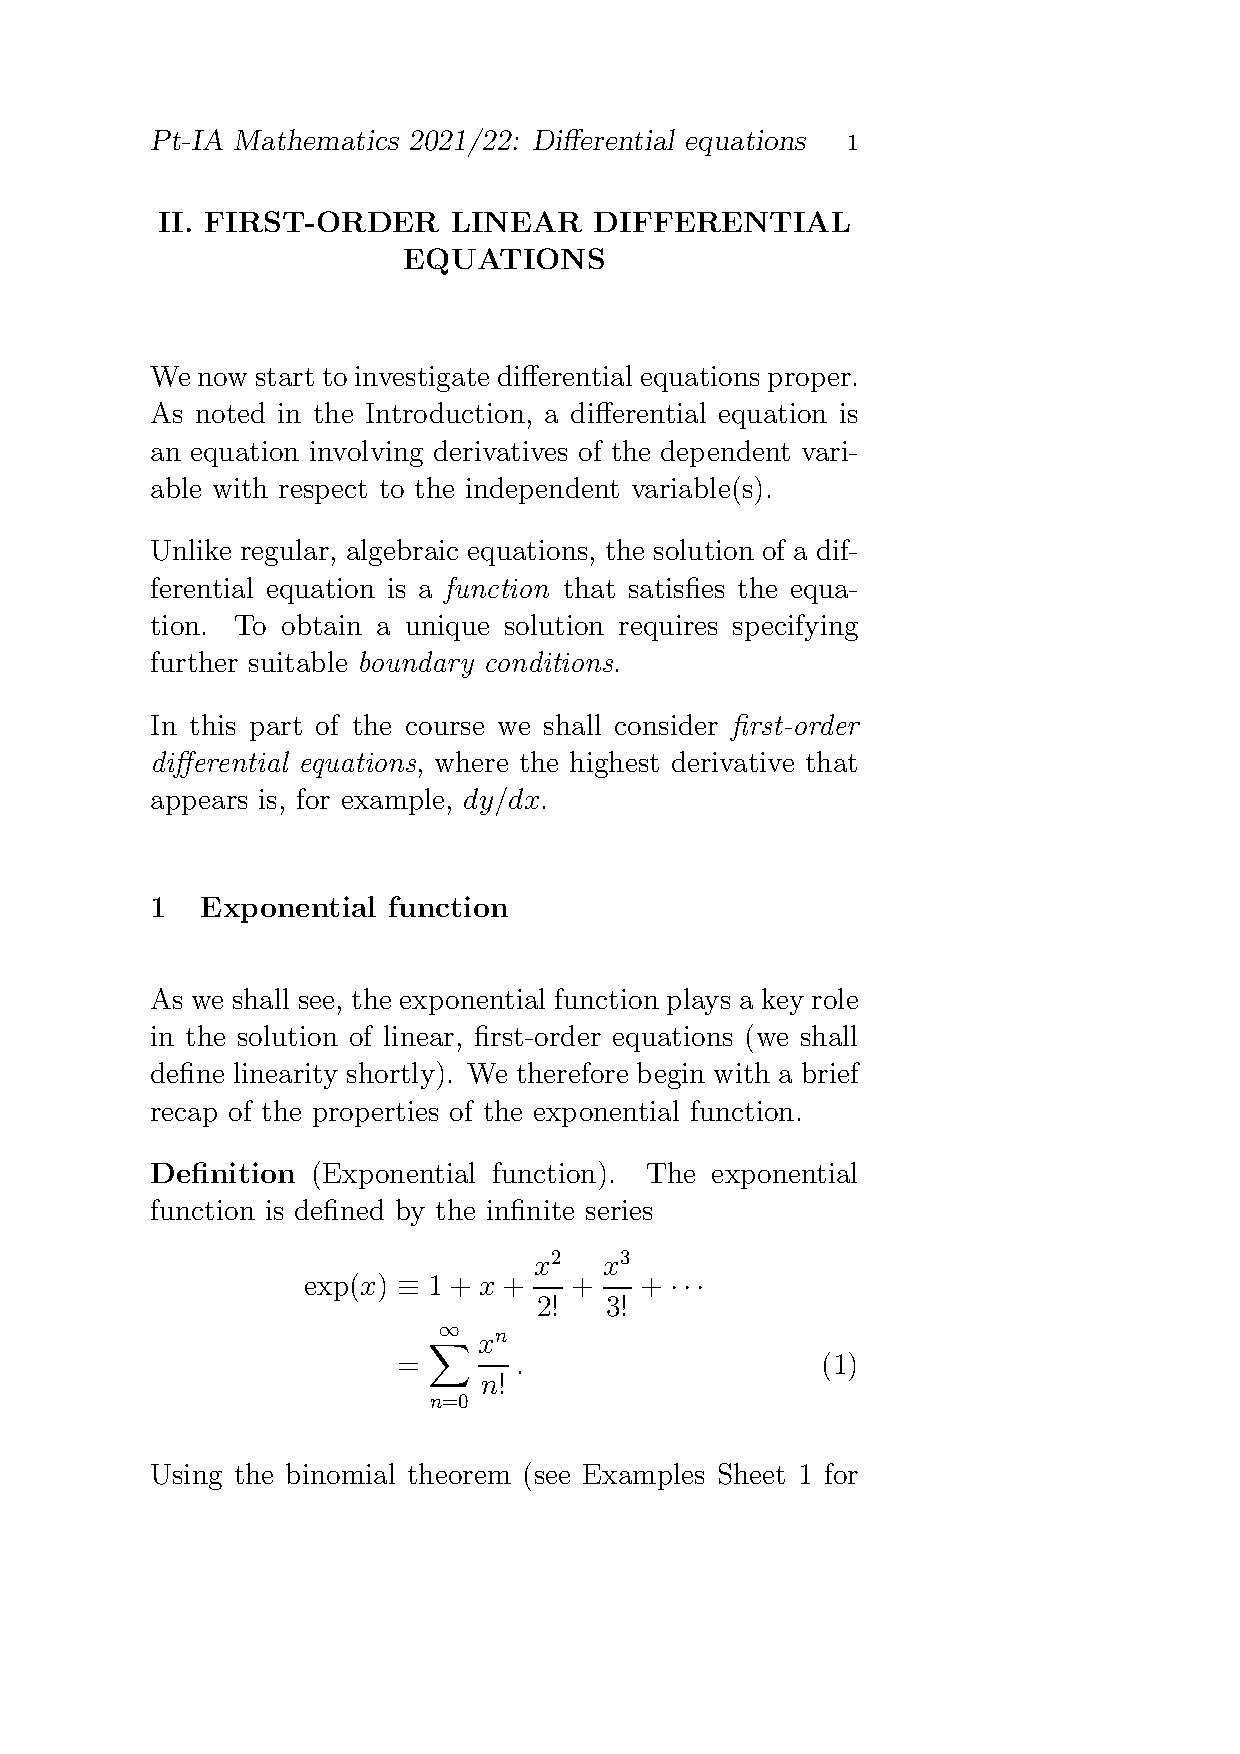
\includepdf[pages=-, addtotoc={ 1,section,1,First-Order Linear Differential Equations,1}]{First-Order Linear Differential Equations - Topic 2.pdf}

\subsection{Extra}

\begin{align*}
    \exp \left(x_1 \right) \exp \left(x_2 \right) &= \lim_{k \to \infty} \left(1 + \frac{x_1}{k}\right)^k \left(1 + \frac{x_2}{k}\right)^k \\
    &= \lim_{k \to \infty} \left[ \left(1 + \frac{x_1}{k}\right)\left(1 + \frac{x_2}{k}\right) \right]^k \\
    &= \lim_{k \to \infty} \left[ 1 + \frac{x_1 + x_2}{k} + \frac{x_1 x_2}{k^2} \right]^k \\
    &= \lim_{k \to \infty} \left[ 1 + \binom{k}{1} \frac{1}{k} \left(x_1 + x_2 + \frac{x_1 x_2}{k} \right) + \ldots \right]^k \\
    &= \lim_{k \to \infty} \left[ 1 + \left( x_1 + x_2 \right) + \frac{\left( x_1 + x_2 \right)^2}{2!} + \ldots \right] \\
    &= \exp \left( x_1 + x_2 \right)
\end{align*}

% \includepdf[pages=-, addtotoc={ 1,section,1, Nonlinear, First-Order Differential Equations, 1}]{Nonlinear, First-Order Differential Equations - Topic 3.pdf} 

\includepdf[pages=-, addtotoc={ 1,section,1, Nonlinear First-Order Differential Equations, 1}]{Nonlinear First-Order Differential Equations.pdf} % Can't have commas in filename.

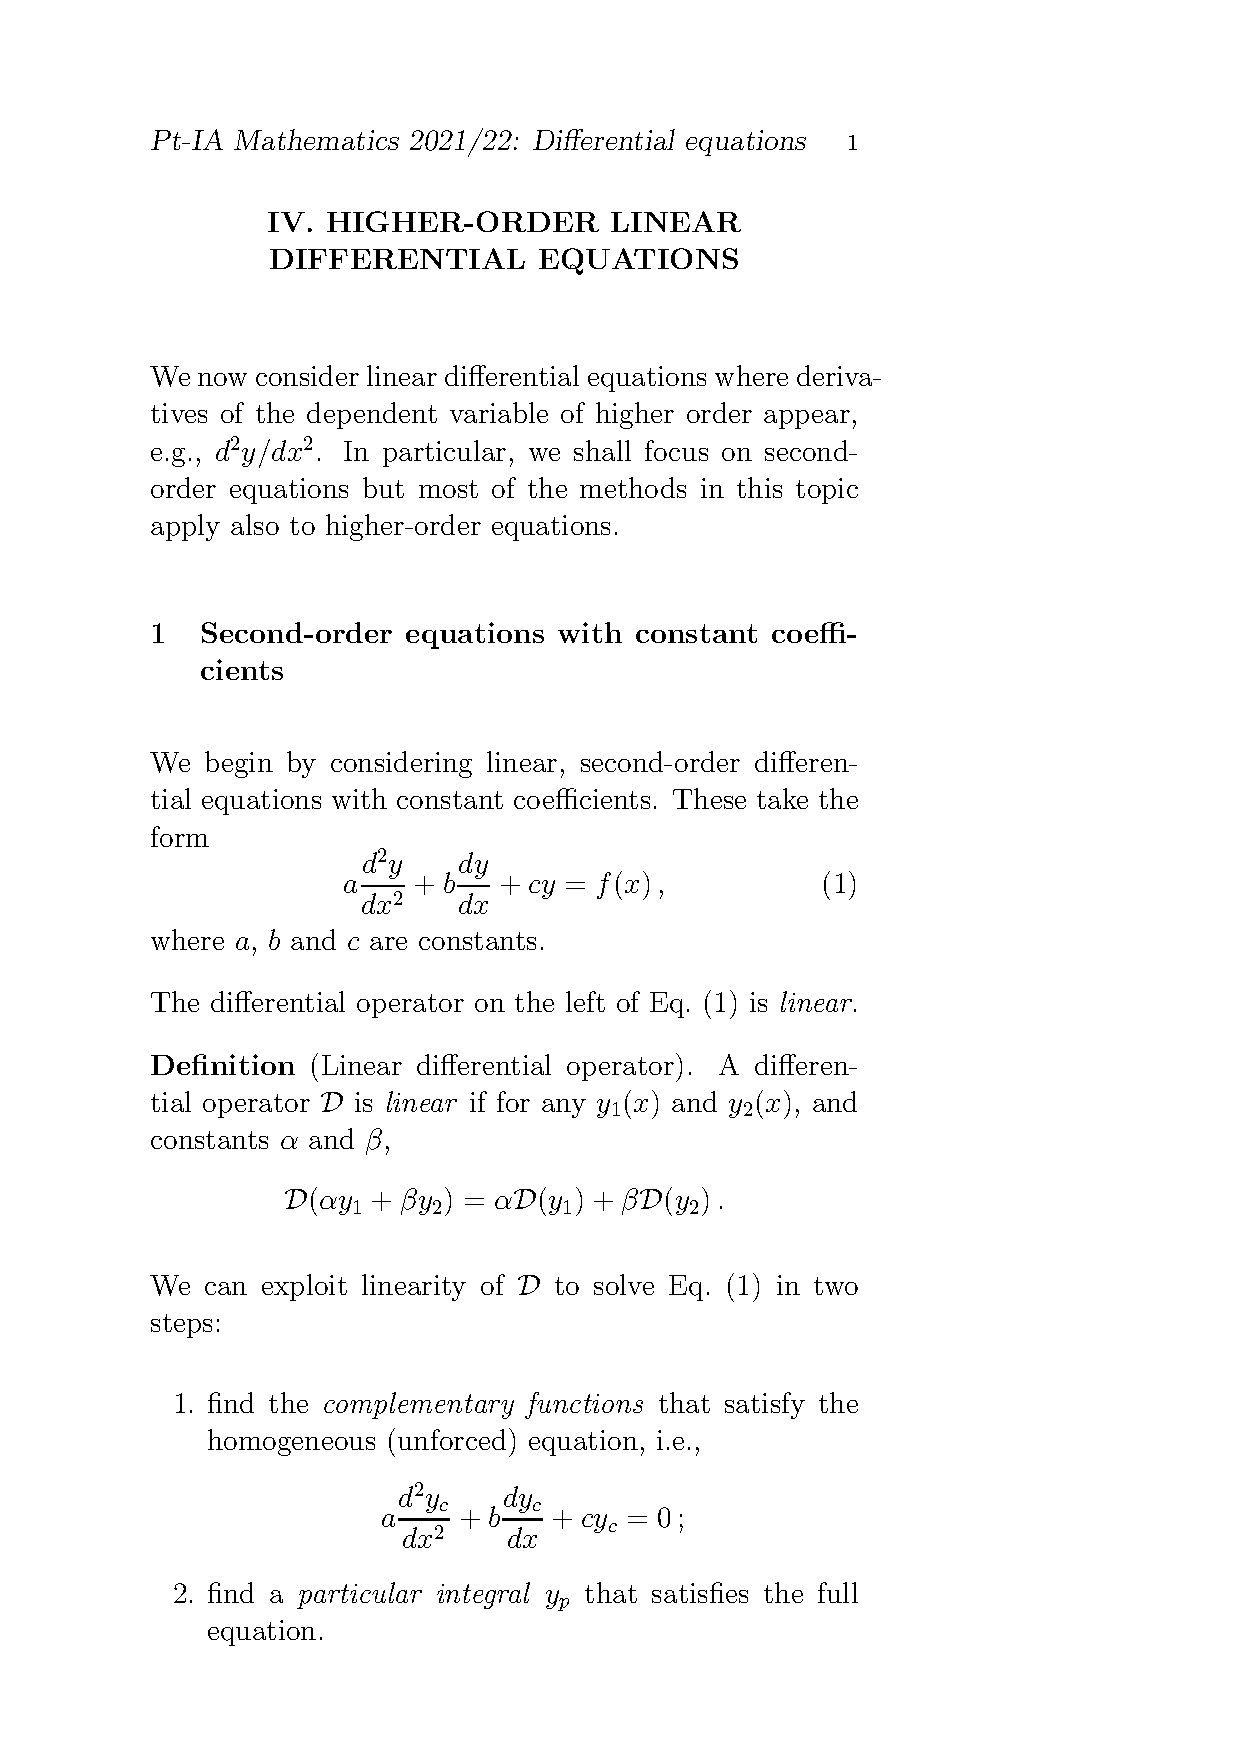
\includepdf[pages=-, addtotoc={ 1,section,1,Higher-Order Linear Differential Equations, 1}]{Higher-Order Linear Differential Equations - Topic 4.pdf} 

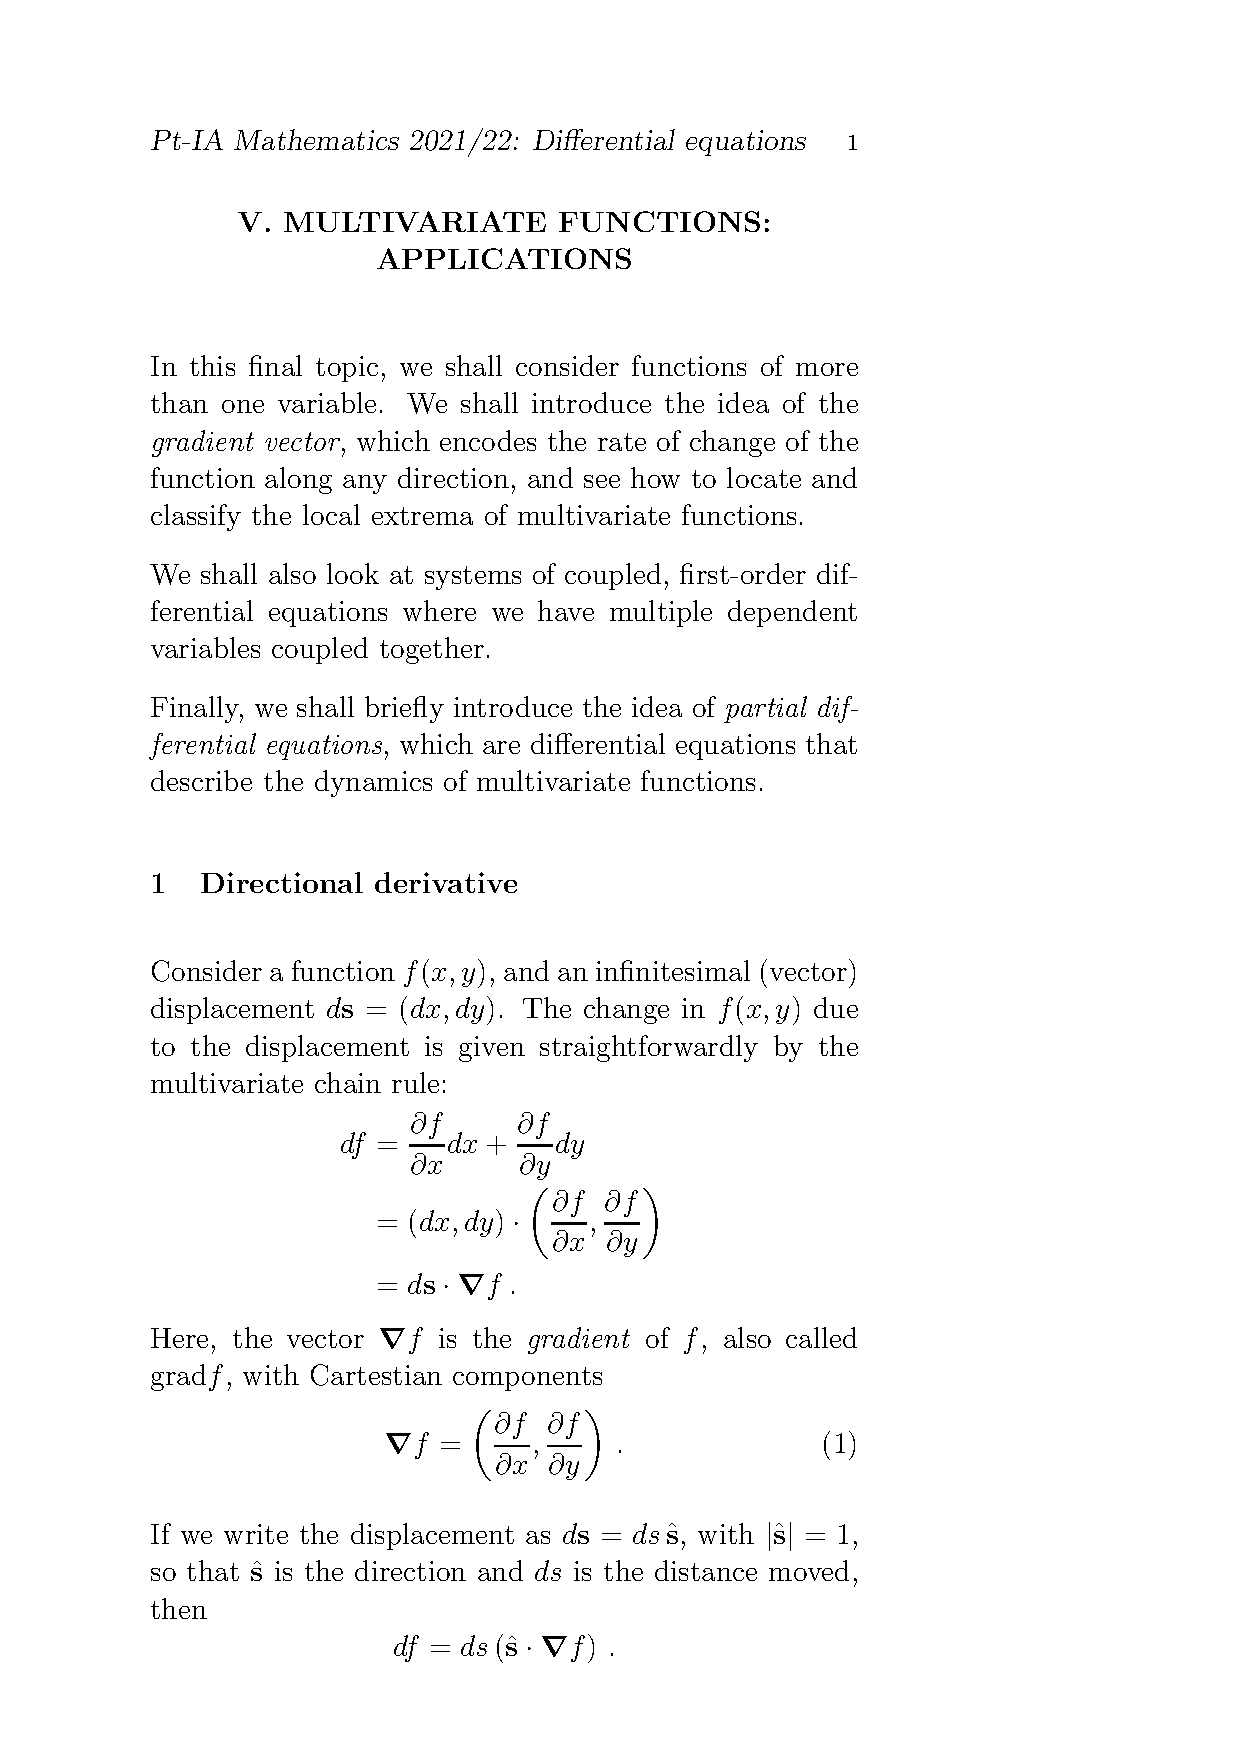
\includepdf[pages=-, addtotoc={ 1,section,1,Multivariate Functions: Applications, 1}]{Multivariate Functions Applications - Topic 5.pdf} 


\end{document}